% vim:encoding=utf8 ft=tex sts=2 sw=2 et:

\documentclass{classrep}
\usepackage[utf8]{inputenc}
\usepackage{fixltx2e}
\usepackage{url}
\usepackage{graphicx}
\usepackage{siunitx}


\studycycle{Informatyka, studia niestacjonarne, inż I st.}
\coursesemester{VI}

%\coursename{hhhhhhhheoretyczna i stosowana}
\coursename{Inteligentna Analiza Danych}
\courseyear{2013/2014}

\courseteacher{mgr inż. Michał Pryczek}
\coursegroup{sobota, 11:15}

\author{
  \studentinfo{Łukasz Ochmański}{183566} \and
  \studentinfo{Przemysław Szwajkowski}{173524}
}

\title{Zadanie 2b: Perceptron Wielowarstwowy}
\svnurl{http://iad-lukasz-ochmanski.googlecode.com/svn/trunk/02}

\begin{document}
\maketitle


\section{Cel}
Celem zadania było zbadanie zależności działania sieci neuronowej od jej struktury.
W zadaniu zmieniano liczbę neuronów wyjściowych, neuronów wejściowych, liczbę warstw ukrytych oraz liczbę neuronów w poszczególnych warstwach.

\section{Wstęp}
W badaniu uwzględniono pięć konfiguracji sieci perceptronowej:
\item
1. 4-3-3
\item
2. 4-4-3
\item
3. 4-3-4-3
\item
4. 4-6-3
\item
5. 4-4-4-4-4-3

\\*

\begin{figure}[ht]
\centering
			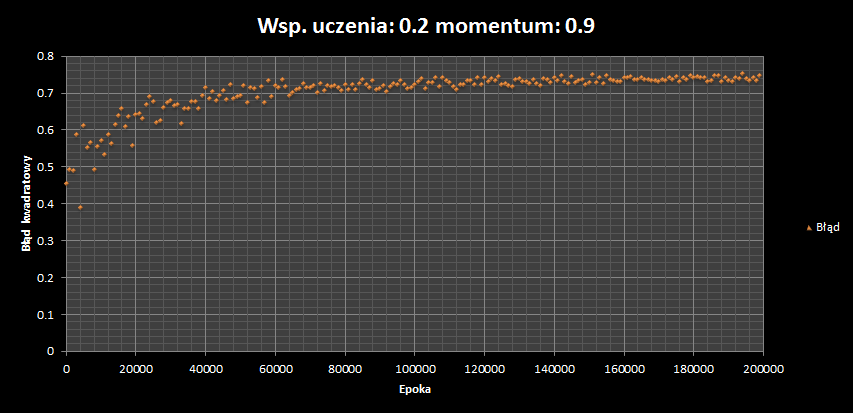
\includegraphics[scale=0.65]{pictures/Iris01.png}
	\caption{Iris data set}
	\label{fig:Iris data set}
\end{figure}

\begin{figure}[ht]
\centering
			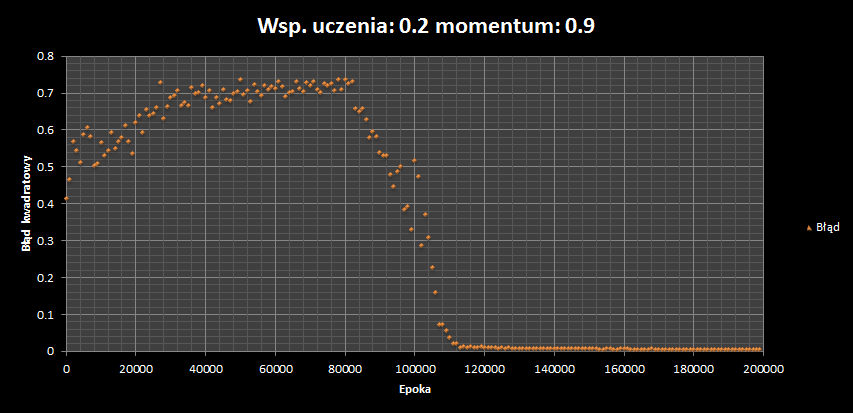
\includegraphics[scale=0.65]{pictures/Iris02.png}
	\caption{Iris data set}
	\label{fig:Iris data set}
\end{figure}

\begin{figure}[ht]
\centering
			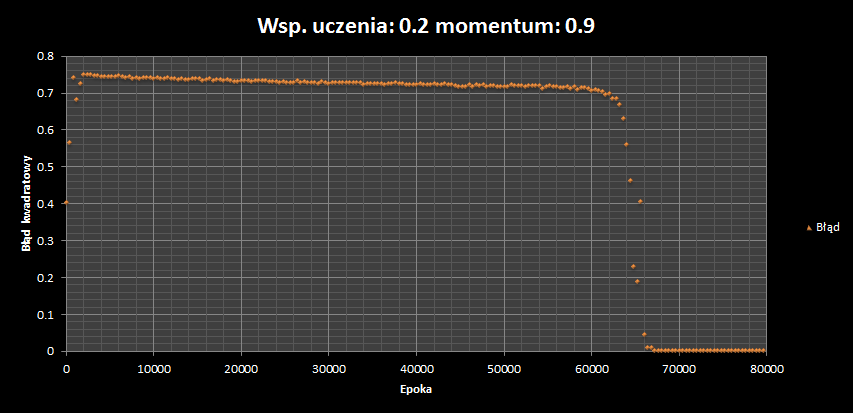
\includegraphics[scale=0.65]{pictures/Iris03.png}
	\caption{Iris data set}
	\label{fig:Iris data set}
\end{figure}

\begin{figure}[ht]
\centering
			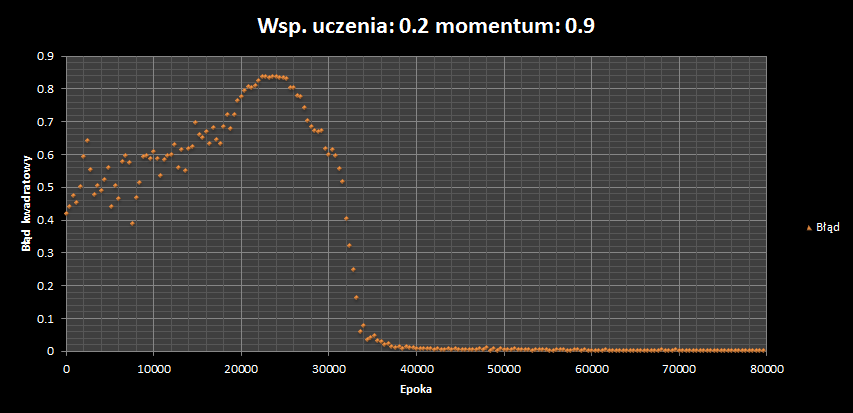
\includegraphics[scale=0.65]{pictures/Iris04.png}
	\caption{Iris data set}
	\label{fig:Iris data set}
\end{figure}

\begin{figure}[ht]
\centering
			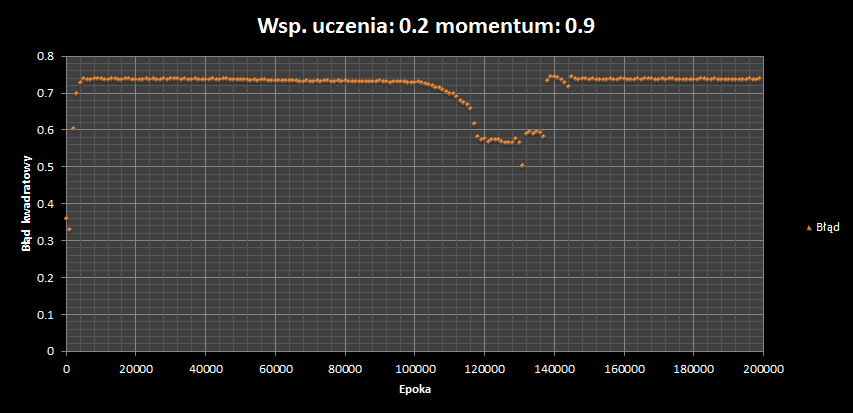
\includegraphics[scale=0.65]{pictures/Iris05.png}
	\caption{Iris data set}
	\label{fig:Iris data set}
\end{figure}

\clearpage

Rysunki 1. - 4. dotyczą zestawu Iris, w którym zbiór treningowy składa się ze 150 testów.
Oczekiwanym wyjściem były odpowiednie wiersze macierzy jednostkowej o wymiarze 3,
przyporządkowane poszczególnym wartością cechy nominalnej (gatunku irysa).
W przypadkach, w których wystąpił problem, dotyczył on tego samego, co mogłoby być
problemem dla człowieka rysującego krzywe podziału w zbiorze Iris - czyli
odróżnianie specyficznych osobników gatunku virginica od versicolor.

Przeprowadzenie aż pięciu testów
służyło porównaniu skuteczności i szybkości otrzymywania zadowalająco
małych błędów globalnych sieci dla różnych liczebności warstw. Wszystkie próby
były wykonywane z wykorzystaniem neuronów obciążających, przy losowym podawaniu
testów w poszczególnych epokach. Aby uczynić wykresy porównywalnymi, różne konfiguracje
testowano przez 200000 epok, lub - jeżeli konfiguracja składała się z wielu neuronów
i dawała dobre wyniki istotnie szybciej - 80000 epok. \\

Test 1. był próbą rozwiązania problemu za pomocą sieci o konfiguracji 4-3-3. Mimo
obecności neuronów obciążających, sieć ta okazała się zbyt uboga aby dokonać poprawnej
klasyfikacji. Po 200000 epokach nauki, jeden z~irysów pozostał klasyfikowany błędnie,
zaś inny - był klasyfikowany zauważalnie mało zdecydowanie. \\

Dodanie czwartego neuronu do warstwy ukrytej znacząco poprawiło szybkość nauki - dzięki
temu w w teście 2. przy stosowanej metodzie przeprowadzania eksperymentów udało się nauczyć sieć
klasyfikacji irysów już w nieco poniżej 120000 epok. Patrząc na wagi drugiej
i trzeciej warstwy można zaobserwować, że dla ostatnich trzech wyjść warstwy drugiej
wagi w pierwszym neuronie warstwy trzeciej są bliskie zeru, a w warstwie drugiej są liczbami
przeciwnymi do wag w warstwie trzeciej.
Neurony 2-4 różnią się między sobą, lecz z punktu widzenia warstwy wyjściowej wystarczyłoby rozważać pewną
sumę ważoną ich wyjść i korzystać z pojedynczej liczby wspólnej dla wszystkich neuronów warstwy wyjściowej.
Poza tą liczbą oczywiście potrzebny jest neuron 2.1 oraz bias. Może
zatem konfiguracja 4-2-3 z biasem byłaby wystarczająca? Otóż jak pokazuje wykres 1., cztery neurony
warstwy ukrytej są jednak potrzebne aby proces nauki mógł się odbyć, nawet jeśli
w końcowym procesie nauczania znaczenie faktu, że neurony 2-4 są różne zostaje zatarte. \\

Wykres 3. pokazuje sprawność naszej implementacji w przypadku dodania kolejnych warstw.
Pomimo, że dane już w pierwszej warstwie ukrytej muszą być przepuszczone przez zaledwie
trzy neurony, ze względu na rozmiar drugiej warstwy ukrytej proces uczenia nie sprawia
problemu, an nawet trwa prawie dwa razy mniej epok niż na wykresie 2 (czyli niecałe 70000 epok).
Zatem dane przechodzące przez 3 neurony w pewnej warstwie ukrytej bez
problemu mogą posłużyć do klasyfikacji irysów, mimo że nie udało się to na rysynku 1.
Mimo znacznego zmniejszenia liczby epok w porównaniu do rysynku 2., należy pamiętać,
że czas obliczeń potrzebnych do przebiegu epoki wzrósł ze względu na dodanie
kolejnej warstwy neuronów. \\

Aby osiągnąć przyspieszenie nauki sieci, zamiast dodawać kolejne warstwy, można także
dodać nadmiarowe neurony w warstwie ukrytej. Sieć 4-6-3 (rysunek 4.) nauczyła się
klasyfikować irysy w mniej niż 40000 epok, co stanowi najlepszy z uzyskanych wyników.
Duża liczba neuronów nie pozostaje jednak bez wpływu na czas obliczeń, więc nadal
można się zastanawiać, która ze struktur - niniejsza, zastosowana na rysunku 2., czy może na rysynku 3.
- jest najlepszym rozwiązaniem problemu. Może to zależeć na przykład od tego, czy chcemy
skoncentrować się na minimalizacji czasu obliczeń, czy może liczby neuronów i
związanego z nią zużycia pamięci. Dla tak małych sieci znaczenie tego jest znikome,
ale gdyby dwie liczne warstwy sąsiadowały ze sobą, zużycie pamięci wzrosłoby znacznie
- wtedy może opłacić się rozważanie utworzenia dwóch warstw ukrytych. \\

Rysunek 5. stanowi eksperyment na temat tego, do czego może doprowadzić znaczna
przesada z liczbą warstw ukrytych. Mimo upływu 200000 epok i~chwilowego
zmniejszenia maksymalnego błędu globalnego w epoce, sieć ta nie zdołała
nauczyć się całego zbioru danych - jeden z irysów pozostał klasyfikowany błędnie.
Chwilowy spadek, a później - ponowny wzrost maksimum błędu (czyli błędu
na problematycznym irysie) jest zjawiskiem podobnym do przeuczenia - jednakże
w tym przypadku całkowite nauczenie sieci zbioru treningowego nie
nastąpiło wcale. \\

\section{Wnioski}
Podsumowując, na podstawie wyników i przedstawionej powyżej ich interpretacji
wyciągnęliśmy następujące wnioski:

\begin{itemize}
\item Jeżeli w sieci występują warstwy składające się z niewielkiej liczby neuronów,
użycie obciążenia jest nie tylko ułatwieniem, ale wręcz koniecznością.
\item Umiarkowane podwyższanie współczynnika nauki oraz momentum pozwala przyspieszać
proces nauczania.
\item W przypadku spodziewanej dużej liczby epok, dobrze sprawdza się umiarkowany współczynnik
nauki i duży współczynnik momentum (np. nauka $0,2$ i momentum $0,9$) - właśnie przy
takich współczynnikach udało nam się dokonać klasyfikacji zbioru Iris.
\item Zastosowanie współczynnika momentum pozwala uniknąć występowania lokalnych minimów,
oraz wygładza przebieg nauki dla dużych zbiorów testowych. Jego zastosowanie jest korzystne
zwłaszcza podczas treningu sieci on-line, oraz w sytuacjach w których mogłoby dojść do przeuczenia sieci.
Ze względu na charakter wpływu momentum na zmiany wag neuronu, często określa się je jako bezwładność wagi.
\item Dla skomplikowanego zbioru treningowego często problemem może się okazać
pewien pojedynczy test - nie jest to za każdym razem ten sam test, ale zawsze
znajduje się on blisko płaszczyzn separacji, które można by sobie próbować wyobrazić.
\item Nawet jeżeli stosowane jest obciążenie, to jeżeli któraś warstwa ukryta
będzie zawierała zbyt mało neuronów, rozróżnienie wymaganej liczby
unikalnych wyjść może okazać się niemożliwe.
\item Odmienny od powyższego problem polega na tym, że sieć po prostu może
być zbyt uboga, aby proces nauki przebiegał skutecznie. Nawet jeżeli
po ukończonej nauce część neuronów okazuje się być nadmiarowa,
są one potrzebne do prawidłowego przebiegu procesu nauki.
\item Dodanie dodatkowej warstwy ukrytej może poprawić szybkość uczenia, ale
jeszcze lepiej jest dodać równoległe neurony do istniejącej warstwy. Jedynym
argumentem za dodatkowymi warstwami może być zużycie pamięci, które maleje
gdy rozległa warstwa zostaje rozbita na dwie mniejsze (o ile nie okażą się
one z kolei zbyt ubogie, aby rozróżnić wymaganą liczbę różnorodnych wyjść).
\item Utworzenie zbyt wielu warstw ukrytych uniemożliwia dostosowanie sieci
do kłopotliwych testów ze zbioru treningowego.
\end{itemize}

\begin{thebibliography}{0}
  \bibitem{l2short} \textsl{Ryszard Tadeusiewicz} - Sieci neuronowe, \textsl{Wyd. 2., Warszawa 1993}
  \bibitem{l2short} ``Learning and neural networks'' [\url{http://en.wikiversity.org/wiki/Learning_and_neural_networks}]
  \bibitem{l2short} UCI Machine Learning Repository \textsl{Iris Data Set}
\end{thebibliography}
\end{document}